\section{Método}\label{sec:metodo}

\textbf{Modelos.} Comparamos dos formas de estimar el rendimiento promedio de un municipio.
\begin{itemize}
\item \textbf{Kriging de vecinos.} Estima un municipio con un promedio ponderado del rendimiento de los municipios
con SIAP, donde los más próximos pesan más. Los pesos no se fijan a mano. Se aprenden de los datos midiendo qué tanto
se parecen los rendimientos de dos municipios según la distancia que los separa~\cite{rasmussen2006,oliver2014}. Es la
base a superar porque no usa ambiente.
\item \textbf{Modelos ambientales simples.} Regresiones lineales con una o dos variables elegidas por lo que se sabe
del cultivo. La principal usa la Tmax de julio y agosto, porque en la cebada unos pocos días de calor sobre la espiga
durante el llenado reducen el peso del grano~\cite{passarella2002}.
\end{itemize}
También probamos modelos con 14 variables de clima, terreno y suelo.

\textbf{Detalle del kriging.} Es un proceso gaussiano sobre las coordenadas de los centroides municipales. La
covarianza entre dos municipios a distancia $d$ es una Matérn de suavidad $\nu = 3/2$ más ruido blanco,
\[
k(d) = \sigma^2\Bigl(1 + \tfrac{\sqrt{3}\,d}{\ell}\Bigr)e^{-\sqrt{3}\,d/\ell} + \tau^2\,\mathbf{1}[d = 0].
\]
El ruido $\tau^2$ representa el error propio del promedio de cada municipio. La longitud de correlación $\ell$ y las
varianzas $\sigma^2$ y $\tau^2$ se estiman por máxima verosimilitud en cada partición, solo con los municipios de
entrenamiento. La media es una constante igual al promedio de los promedios municipales. La optimización parte de
$\ell = 30$\,km con cotas de 2 a 500\,km, usa tres inicios y semilla fija. El ruido tiene una cota inferior, la mitad
de la mediana de la varianza de la media de cada municipio entre la varianza entre municipios. Con zona de exclusión
de 50\,km, $\ell$ promedia 35\,km (de 12.6 a 85.7), $\sigma^2 = 0.16$ y $\tau^2 = 0.05$ (t/ha)$^2$. En 24.5\,\% de las
particiones el ruido queda en su cota inferior, así que esa cota condiciona el resultado cuando hay pocos municipios.

\textbf{Tmax.} Es la temperatura máxima diaria promedio de julio y agosto sobre la agricultura de temporal del
municipio, promediada de 2003 a 2025. Sale de CHIRTS-ERA5~\cite{chirts,verdin2020} y no del SIAP, así que existe para
cualquier municipio, tenga o no datos de rendimiento. Los rendimientos del SIAP solo sirven para ajustar la
regresión, es decir, para saber cuánto cambia el rendimiento por cada grado de Tmax.

\textbf{Modelo final.} Combina los dos anteriores en dos pasos. Primero la regresión con Tmax da un rendimiento para
cada municipio. Después calculamos su error en cada municipio con SIAP, la diferencia entre el rendimiento observado y
el predicho, y aplicamos el kriging a esos errores en lugar de al rendimiento. Si los vecinos de un municipio rinden
más de lo que su Tmax predice, por manejo, variedad o suelo, el municipio recibe parte de esa corrección. Lejos de
municipios con SIAP la corrección se acerca a cero y queda solo la predicción por Tmax. El kriging de estos errores se
ajusta igual que el anterior. Su longitud de correlación baja a unos 14\,km y su ruido a 0.014\,(t/ha)$^2$, porque
tras quitar la Tmax queda una correlación espacial muy local. Su ruido toca la cota inferior en 34\,\% de las
particiones con zona de exclusión.

\textbf{Validación.} Agrupamos los 100 municipios en 20 zonas con el método de k-medias sobre sus coordenadas y
predecimos una zona a la vez sin usar sus datos. Una validación espacial evita que la autocorrelación infle el
desempeño~\cite{roberts2017,ploton2020}. Para simular un lugar realmente nuevo quitamos además los municipios a menos
de $B = 50$\,km de la zona (Fig.~\ref{fig:validacion}). Con $B = 0$ solo se deja fuera la zona. Repetimos todo 10
veces con agrupamientos distintos. Las repeticiones comparten los mismos 100 municipios, así que no son pruebas
independientes. Para medir la incertidumbre remuestreamos los municipios 4\,000 veces (bootstrap) y reportamos
intervalos de 95\,\%.

\textbf{Error.} Usamos la raíz del error cuadrático medio (RMSE) en t/ha entre el rendimiento promedio predicho
$\bar p_i$ y el observado $\bar y_i$ de cada municipio $i$,
\[
\mathrm{RMSE} = \sqrt{\frac{\sum_i w_i\,(\bar p_i - \bar y_i)^2}{\sum_i w_i}}.
\]
El peso $w_i$ es la superficie sembrada media del municipio, en forma lineal. Va de 50 a 21\,136\,ha, con mediana de
687\,ha. Los 10 municipios con más superficie suman el 51\,\% del peso y el tamaño efectivo de muestra
$1/\sum_i (w_i/\sum_j w_j)^2$ es 28 de 100. Ponderamos porque FIRA opera donde hay más superficie. Las regresiones se
ajustan con mínimos cuadrados con los mismos pesos y el kriging no usa pesos. También reportamos el RMSE sin pesos
entrenando sin pesos las regresiones, para que la comparación sea justa.

\textbf{Regla de decisión.} La fijamos antes de correr los experimentos. Un modelo ambiental sustituye al kriging si gana
en al menos 7 de las 10 repeticiones y si su ventaja desaparece al revolver las variables entre municipios.

\begin{figure}[!tbp]
\centering
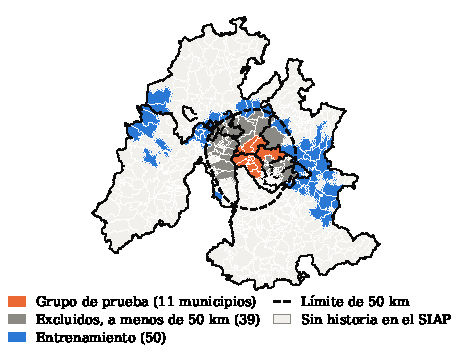
\includegraphics[width=\columnwidth]{g_validacion}
\caption{Una partición de la validación. El modelo se entrena sin los municipios grises y predice los naranjas, como
si fueran un lugar sin datos del SIAP a menos de 50\,km.}
\label{fig:validacion}
\end{figure}
